\section{Application Examples}

\subsection{Identification of minor oxides}
    \citet{benaboud2007} showed that the photoelectrochemical characterization 
    is robust for detecting the presence of minor oxides. 
    Alloying elements Fe, Sn and Cr, present in Zircaloy4, form precipitates 
    which can be oxidized and trapped in the zirconia layer during the 
    oxidation process. 
    The oxidized precipitates are therefore minor oxide phases in the zirconia 
    layer. 
     illustrates the photocurrent spectra measured on Zircaloy-4 
    and “pure” zirconium where the strong photocurrent observed at around 5~eV 
    reveals the major oxide i.e. monoclinic zirconia. 
    The photocurrent at energy lower than 5 eV is not null and reveals the 
    presence of minor oxides even in “pure” zirconium despite the very low 
    concentration of impurities. 
    The slope changes provided an estimation of the band gaps where the author 
    identified the presence of hematite, chromia and a solid solution of 
    $(Fe_xCr_{1-x})O_3$. 
    The identification is made based on data available in literature \citep{morrison1980}.

    \renewcommand{\coef}{0.45}
    \begin{figure}[h]
        \centering
        \begin{subfigure}{\coef\textwidth}
            \centering
            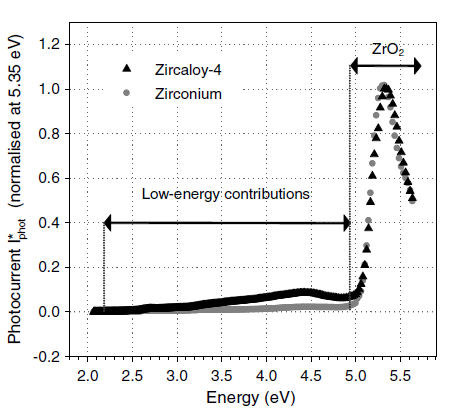
\includegraphics[width=\textwidth]{./src/figures/Benaboud2007-Fig4.png}
            \caption{}
            \label{fig_benaboud_minor_oxides_a}
        \end{subfigure}
        \begin{subfigure}{\coef\textwidth}
            \centering
            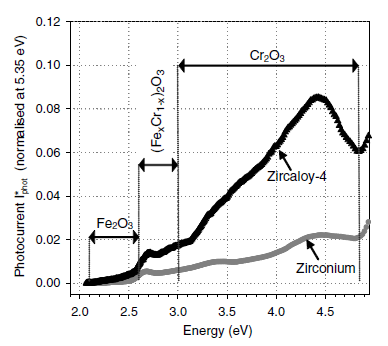
\includegraphics[width=\textwidth]{./src/figures/Benaboud2007-Fig5.png}
            \caption{}
            \label{fig_benaboud_minor_oxides_b}
        \end{subfigure}
        
        \caption{Photocurrent spectra measured on zirconia oxide layer formed on 
        Zircaloy4 and “pure” zirconium oxidized for 1h at 470°C in oxygenated 
        atmosphere\citep{benaboud2007}: a) complete spectrum b) close-up view on the minor contributions.}
        \label{fig_benaboud_minor_oxides}
    \end{figure}



\subsection{Identification of semiconduction type}
    \citet{loucif2013} showed the effect of hydrogen pressure on 
    the semiconduction type on Nibased alloy 600 oxidized in simulated PWR. 
    Figure~\ref{fig_loucif_sctype_a} shows a “V-shape” of the normalized photocurrent which 
    reveals an isolating behavior of the oxide layer at high hydrogen pressure. 
    Figure~\ref{fig_loucif_sctype_b} shows a monotonous increase of the 
    normalized photocurrent towards more anodic potentials which reveals 
    n-type semiconduction.

    \renewcommand{\coef}{0.45}
    \begin{figure}[h]
        \centering
        \begin{subfigure}{\coef\textwidth}
            \centering
            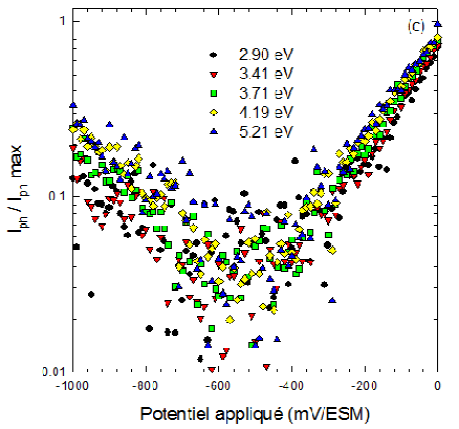
\includegraphics[width=\textwidth]{./src/figures/Loucif2012-Fig3-18.png}
            \caption{}
            \label{fig_loucif_sctype_a}
        \end{subfigure}
        \begin{subfigure}{\coef\textwidth}
            \centering
            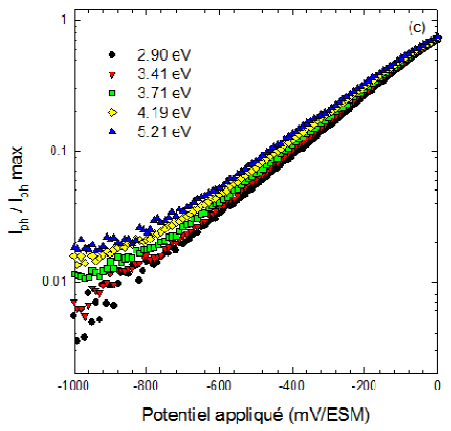
\includegraphics[width=\textwidth]{./src/figures/Loucif2012-Fig3-19.png}
            \caption{}
            \label{fig_loucif_sctype_b}
        \end{subfigure}
        
        \caption{Photocurrent with respect to the potential for an 
        Ni-based alloy 600 polished and oxidized in simulated PWR 
        for 500~h \citep{loucif2013}: a) $P_{H_2}$=6.5~bar, b) $P_{H_2}$=0.05~bar.}
        \label{fig_loucif_sctype}
    \end{figure}



\subsection{High temperature PEC}
    The majority of photoelectrochemical characterizations are performed at 
    room temperature in simple glass/Plexiglas cells where the signal/noise 
    ratio is very good. High temperature photoelectrochemical characterizations 
    require sophisticated metallic cells and transparent windows 
    able to withstand the arch environment. 
    Despite the need to improve the signal/noise ratio, the feasibility of 
    the in-situ photoelectrochemical characterizations was demonstrated by 
    \citet{bojinov2002} in 2002 and more recently by \citet{skocic2016} in 2015 
    as shown in figures~\ref{fig_bojinov_ht} and \ref{fig_skocic_phd}.

    \renewcommand{\coef}{0.45}
    \begin{figure}[h]
        \centering
        \begin{subfigure}{\coef\textwidth}
            \centering
            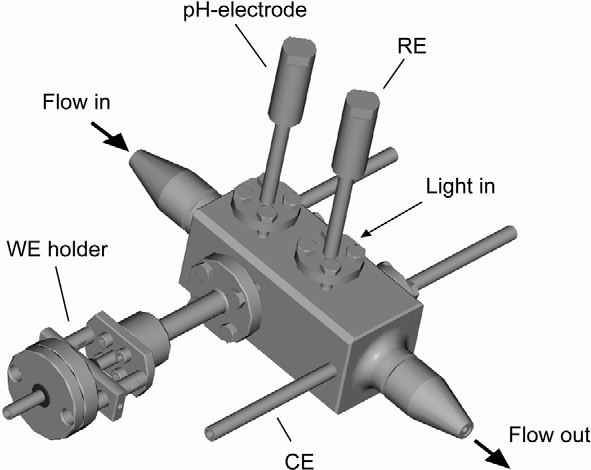
\includegraphics[width=\textwidth]{./src/figures/Bojinov_2002_Fig1.png}
            \caption{}
            \label{fig_bojinov_ht_a}
        \end{subfigure}
        \begin{subfigure}{\coef\textwidth}
            \centering
            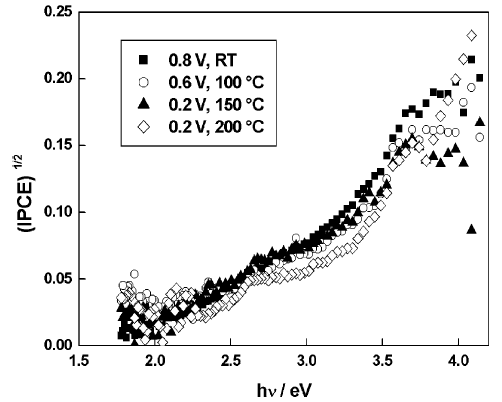
\includegraphics[width=\textwidth]{./src/figures/Bojinov_2002_Fig5b.png}
            \caption{}
            \label{fig_bojinov_ht_b}
        \end{subfigure}
        
        \caption{a) Schematic representation of the metallic cell developed
        by \citet{bojinov2002}. 
        b) Photocurrent spectra performed on iron oxides at different 
        temperatures (up to 200°C) obtained by \citet{bojinov2002}.}
        \label{fig_bojinov_ht}
    \end{figure}



    \renewcommand{\coef}{0.45}
    \begin{figure}[h]
        \centering
        \begin{subfigure}{\coef\textwidth}
            \centering
            \includegraphics[width=\textwidth]{./src/figures/skocic2015-1.png}
            \caption{}
            \label{fig_skocic_phd_cell}
        \end{subfigure}
        \begin{subfigure}{\coef\textwidth}
            \centering
            \includegraphics[width=\textwidth]{./src/figures/skocic2015-2.png}
            \caption{}
            \label{fig_skocic_phd_htpec}
        \end{subfigure}
        
        \caption{a) Schematic view of the photoelectrochemical cell developed by \citet{skocic2016}. 
        b) Photocurrent energy spectra of an X750 specimen recorded at room
        temperature and in 280°C/80 bar water \citep{skocic2016}}
        \label{fig_skocic_phd}
    \end{figure}
